\documentclass{llncs}
\usepackage{geometry}
%\geometry{letterpaper}                   % ... or a4paper or a5paper or ...
\usepackage{graphicx}
\usepackage{xspace}
\usepackage{amssymb} 
\usepackage{epstopdf}
\usepackage{graphicx,color}
  
  
\usepackage{datatool}
\usepackage{tikz}
\usepackage{pgfplots}
\usepackage{pgfplotstable}
\usetikzlibrary{patterns}
\usepackage{lscape}
\usepackage{subfig}
\usepackage{booktabs} % Linhas horizontais para tabelas
%% The amssymb package provides various useful mathematical symbols
\usepackage{amssymb}
%% The amsthm package provides extended theorem environments
%% \usepackage{amsthm}
\usepackage{marginnote}
\newcommand{\daniel}[1]{\marginnote{\textcolor{red}{\textbf{Daniel: }#1}}}
\newcommand{\idaniel}[1]{\marginpar{\textcolor{red}{\textbf{Daniel: }#1}}}

\newcommand{\placido}[1]{\marginnote{\textcolor{blue}{\textbf{Pl\'acido:
}#1}}}
\newcommand{\iplacido}[1]{\marginpar{\textcolor{blue}{\textbf{Pl\'acido:
}#1}}}

\begin{document}

\title{SLA-based Data Integration on Multi-Cloud: A Systematic Mapping Analysis}

\author{
        Daniel A. S. Carvalho\inst{1}, 
        Nadia Bennani\inst{2}, 
        Chirine Ghedira\inst{1}, 
        Pl\'acido A. Souza Neto\inst{3}, 
        Genoveva Vargas-Solar\inst{4}
 		}


\institute{
		Universit\'e Jean Moulin, Lyon 3 MAGELLAN, IAE -- France \\
			\email{daniel.aguiar-da-silva-carvalho@etu.univ-lyon3.fr, chirine.ghedira-guegan@univ-lyon3.fr}
		\and
		CNRS INSA-Lyon, LIRIS, UMR5205 -- France\\
			\email{nadia.bennani@insa-lyon.fr}
		\and
		Instituto Federal do Rio Grande do Norte, Natal -- Brazil \\
			\email{placido.neto@ifrn.edu.br}
		\and
		CNRS, LIG-LAFMIA, Saint Martin d'H\`eres -- France \\
			\email{genoveva.vargas@imag.fr}
		}
		
\maketitle
  
\begin{abstract}

\end{abstract}

\keywords{Systematic Mapping, Service Level Agreement, Data Integration, Multi-cloud Environment.}

\section{Introduction}
\label{sec:intro}

%\idaniel{Doing Nadia's request, I've checked for works regarding our three keywords and also their variations and I didn't find anything. But I found one using Grid "SLA-Guided Data Integration on Database Grids".}

The emergence of new architectures like the cloud opens new opportunities to data processing. 
The possibility of having unlimited access to cloud resources and the ``pay as U go'' model make it possible to change the hypothesis for processing big  data collections.  Instead of designing processes and algorithms taking into consideration  limitations on resources availability, the cloud sets the focus on the economic cost implied of using resources and producing results by parallelizing their use while delivering data under subscription oriented cost models.
 
Integrating and processing heterogeneous Big Data, calls for efficient methods for correlating, associating, filtering them taking into consideration their ``structural'' characteristics (due to variety) but also their quality (veracity), e.g., trust, freshness, provenance, partial or total consistency. 
Existing data integration techniques have to be revisited considering weakly curated and modeled data sets. This can be done according to quality of service requirements expressed by their consumers and Service Level Agreement (SLA) contracts exported by the cloud providers that host  Big Data and deliver resources for executing the associated management processes.

However, it is not an easy task to completely fulfill   SLA contracts particularly because they have to use several cloud providers to integrate the data they require under the conditions they expect.
Naturally, a collaboration between cloud providers becomes necessary~\cite{036} but this should be done in a user-friendly way, with high degree of transparency. As result, new challenges emerge.

SLA have been widely discussed in the cloud computing context. ...

Data Integration...


Our work addresses big data collections integration  in a multi-cloud hybrid context guided by user preferences statements and SLA contracts exported by different cloud providers. The objective is to propose an SLA guided continuous data provision and integration system exported as a DaaS by a cloud provider adapted to the vision of the economic model of the cloud such as accepting partial results delivered on demand or under predefined subscription models that can affect the quality of the results; accepting specific data duplication that can respect privacy but ensure data availability; accepting to launch a task that contributes to an integration on a first cloud whose SLA verifies a QoS require



In this paper, we propose an analysis about the problem of integrating data in multi-cloud environments taking into consideration Service Level Agreement. 
The methodology defined in~\cite{SM:Petersen:2008} presents some guidelines to
performing a systematic mapping review in software engineering research
context. The systematic mapping is a defined method to build
a classification of a field of interest. The results analysis focuses on
frequencies of publications for categories (facets).  

The process workflow describes five interdependent tasks: \textit{(i)}
\textbf{definition of research question} to define the \textit{research scope}; \textit{(ii)} textbf{conduct search} in order to retrieve \textit{all candidate papers}. Those papers are selected applying a query which
express the research interest to scientific databases; \textit{(iii)}
\textbf{screening of papers} to select the \textit{relevant papers} to answer the research
question based on a inclusion and exclusion criteria; \textit{(iv)}
\textbf{keywording using abstracts} to identify terms that helps on developing the
\textit{classification scheme} (mapping categories to classify the papers); and
\textit{(v)} \textbf{fata extraction and mapping process} to sort the relevant
papers into the mapping categories and produce the systematic mapping.


This analysis was done using the Systematic Mapping Methodology~\cite{SM:Petersen:2008}. We propose three facets to determine the main issues to be addressed when SLA, Data Integration and Multi-cloud environments are put together in one research problem.

%The methodology consists in retrieving publications from scientific databases and classifying them in
%categories (called facets). As result we have charts which are used to answer specific research questions
%created in accordance with scientific interests. 


Our final objective is to identify trends and open issues regarding our research topic.

The remaining of this paper is organized as follows. 
The related work is in the section~\ref{sec:rw}. 
section~\ref{sec:sm} describes our steps regarding the methodology.
A quantitative analysis based on the facets is discussed in the section~\ref{sec:qanalysis} and conclusion and final
remarks comes in the section~\ref{sec:conc}.  % Introduction %

%-[BEGIN]-----------------------------------------------------------------------
\section{Related Works}\label{sec:rw}

\subsection{Data integration on multi-cloud environment}

\subsection{Service level agreement}
%-[END]----------------------------------------------------------------------- 


The aim of our bibliographic study using the systematic mapping methodology \cite{SM:Petersen:2008} is to (i) categorize and quantify the key contributions and the evolution of the research done on \textit{SLA-guided
data integration in a multi-cloud environment} and  (ii) discover open issues and limitations of existing works.    
Our study is guided by  three research questions:


\textit{\textbf{RQ1:} Which are the SLA measures that have been mostly
applied  in the cloud?} This question  identifies  the type of
properties used for characterizing and evaluating the services provided  by
different clouds.   
 
\textit{\textbf{RQ2:}  How have published papers on data
 integration evolved towards cloud topics?} This question is devoted to identify the way  data integration problems addressed in the literature started  to include issues introduced by the cloud.

\textit{\textbf{RQ3:} In which way and in which  context has data integration  been linked to Quality of Service (QoS) measures in the literature?} The objective of this question is to understand which QoS measures have been used for evaluating data integration and to determine the conditions in which  specific measures are particularly used.

%--------------------------------------------------------------------------------------------------------------------------------------------
\subsection{Searching and screening  papers} \label{subsec:search}
%--------------------------------------------------------------------------------------------------------------------------------------------

According to our research questions and our expertise in data integration we chose a set of keywords to define a complex query to be used for retrieving papers from four target publication databases: IEEE~\footnote{http://ieeexplore.ieee.org/},
ACM~\footnote{http://dl.acm.org/}, Science Direct~\footnote{http://www.sciencedirect.com/} and
CiteSeerX~\footnote{http://citeseerx.ist.psu.edu/}. We used the following conjunctive and disjunctive general query which was completed with associated terms from a thesaurus and rewritten according to the expression rules of advanced queries in each database: 




\begin{center}
\textit{("Service level agreement"  AND ("Data integration" OR "Database
integration") AND ("Cloud" OR "Multi-cloud "))} \\
\end{center}
\medskip  

We retrieved  a total of 1832 publications. As a result of the filtering process
proposed by the systematic mapping methodology~\cite{SM:Petersen:2008} we excluded 1718 publications.
The number of papers included for building the final collection were 114
publications~\footnote{List of references available in:
https://github.com/danielboni/DEXA-2015-Can-Data-Integration-Quality-be-Enhanced-on-Multi-cloud-using-SLA.git}.

%--------------------------------------------------------------------------------------------------------------------------------------------
\subsection{Defining classification facets}
%--------------------------------------------------------------------------------------------------------------------------------------------

We analyzed the titles and abstracts of the  papers derived in the previous
phase using information retrieval techniques  to identify  frequent
 terms. We used these terms for proposing a classification scheme
consisting of three facets that group dimensions. The following lines define the facets and dimensions of the
classification scheme we propose. 

%.  -   .  .  -   ..  -   ..  -   ..  -   ..  -   ..  -   ..  -   ..  -   ..  -   ..  -   ..  -   ..  -   ..  -   ..  -   ..  -   ..  -   ..  -   ..  -   ..  -   ..  -   ..  -   ..  -   ..  -   .  
\textbf{\textit{Data Integration Environment:}}  
%.  -   .  .  -   ..  -   ..  -   ..  -   ..  -   ..  -   ..  -   ..  -   ..  -   ..  -   ..  -   ..  -   ..  -   ..  -   ..  -   ..  -   ..  -   ..  -   ..  -   ..  -   ..  -   ..  -   ..  -   .  
This facet groups the dimensions that characterize the architectures used for delivering data integration services ({\em data warehouse} and  {\em federated database}) and  architectures used for deploying these services ({\em cloud} and {\em multi-cloud}).

%.  -   .  .  -   ..  -   ..  -   ..  -   ..  -   ..  -   ..  -   ..  -   ..  -   ..  -   ..  -   ..  -   ..  -   ..  -   ..  -   ..  -   ..  -   ..  -   ..  -   ..  -   ..  -   ..  -   ..  -   .  
\textbf{\textit{Data Integration Description:}}
%.  -   .  .  -   ..  -   ..  -   ..  -   ..  -   ..  -   ..  -   ..  -   ..  -   ..  -   ..  -   ..  -   ..  -   ..  -   ..  -   ..  -   ..  -   ..  -   ..  -   ..  -   ..  -   ..  -   ..  -   .  
 This facet groups the dimensions describing the approaches used for describing the databases content in order to  integrate them. Data integration can be done by using {\em meta-data, schema}, and {\em knowledge}.

%.  -   .  .  -   ..  -   ..  -   ..  -   ..  -   ..  -   ..  -   ..  -   ..  -   ..  -   ..  -   ..  -   ..  -   ..  -   ..  -   ..  -   ..  -   ..  -   ..  -   ..  -   ..  -   ..  -   ..  -   .  
\textbf{\textit{Data Quality:}} 
%.  -   .  .  -   ..  -   ..  -   ..  -   ..  -   ..  -   ..  -   ..  -   ..  -   ..  -   ..  -   ..  -   ..  -   ..  -   ..  -   ..  -   ..  -   ..  -   ..  -   ..  -   ..  -   ..  -   ..  -   .  
This facet groups the dimensions  representing data quality measures. Measures can be related directly to data for instance {\em confidentiality, privacy, security, protection and provenance} and to the conditions in which data is integrated and delivered  (i.e., dimension {\em SLA}).           

The original vision of our classification scheme is that of adding the notion of {\em quality} to data integration represented by the facets {\em data quality}
and  {\em SLA}.
With these facets our classification scheme shows the aspects that must be considered when addressing data integration in the cloud  taking into account (i) the quality of data, (ii) the systems that integrate data and (iii) the quality warranties that a data consumer can expect expressed in SLAs.

%------------------------------------------------------------------------------- %
\section{Quantitative Analysis}\label{sec:qanalysis}
%--------------------------------------------------------------------------------% 

This section discusses the quantitative analysis  presented in bubble charts that combine different facets. 
In order to observe the evolution of the publication trends we defined a time screen between the years 1998 and 2014 (see Figure \ref{fig:pubperyear}). SLA has emerged when Cloud issues started to be addressed around 2009. The number of publications has increased as cloud infrastructures have become more popular and accessible. It seems  that data integration is an open issue when it is combined with SLA and cloud trends. Less recent papers seem to be devoted to the way data is described under schemata or knowledge representation strategies. This could be due to the fact that these strategies are consolidated today and  to the emergence of NoSQL approaches with their schema-less philosophy \cite{sadalage2012nosql}. 

\begin{figure}[ht!]
\centering
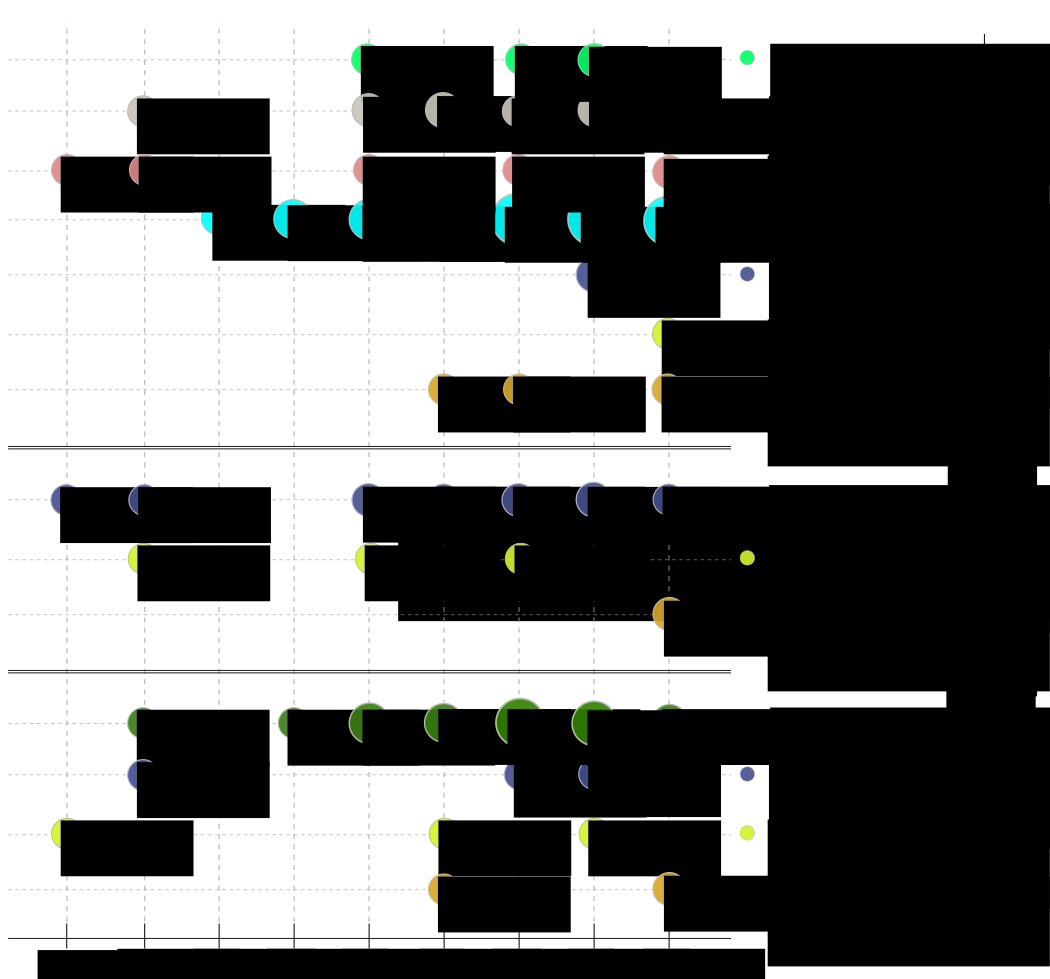
\includegraphics[scale=0.33]{figs/bubble-charts/PublicationsPerYear.pdf} 
\caption{Publications Per Year}\label{fig:pubperyear}
\end{figure}

We combined facets for answering the research questions proposed for guiding our
study. The following lines discuss the answers.
 
%  . .  .  . .  .  . .  .  . .  .  . .  .  . .  .  . .  .  . .  .  . .  .  . .  .  . .  .  . .  .  . .  .  . .  .  . .  .  . .  .  . .  .  . .  .  . .  .  . .  .  . .  .  . .  .
\textbf{\textit{RQ1: Which are the SLA measures that have been mostly applied 
in the cloud?}}
%  . .  .  . .  .  . .  .  . .  .  . .  .  . .  .  . .  .  . .  .  . .  .  . .  .  . .  .  . .  .  . .  .  . .  .  . .  .  . .  .  . .  .  . .  .  . .  .  . .  .  . .  .  . .  .


The facets SLA expression, data integration description and contribution give elements for determining which SLA measures have been applied to the cloud (Figure~\ref{fig:facet1}). 
The resulting bubble chart shows that most contributions propose SLA models and that  \textit{privacy}
and \textit{security} (11 papers - 9.65\%) are the most popular measures considered by SLA models for the cloud. These measures concern the network, information, data protection and confidentiality in the cloud. Most contributions propose SLA models (53 papers - 46.49\%)  but some languages (8 papers - 7.02\%) have also emerged. {\em Data provenance} is also a measure that emerges but only in papers dealing with multi-cloud environments. Data integration is merely addressed by using schemata (12 papers - 10.53\%)  and meta-data (4 papers - 3.51\%) particularly through models (34 papers - 29.82\%) and tools (25 papers - 21.93\%). Still, some works propose surveys (8 papers - 7.02\%).
 
\begin{figure}[ht!]
\centering
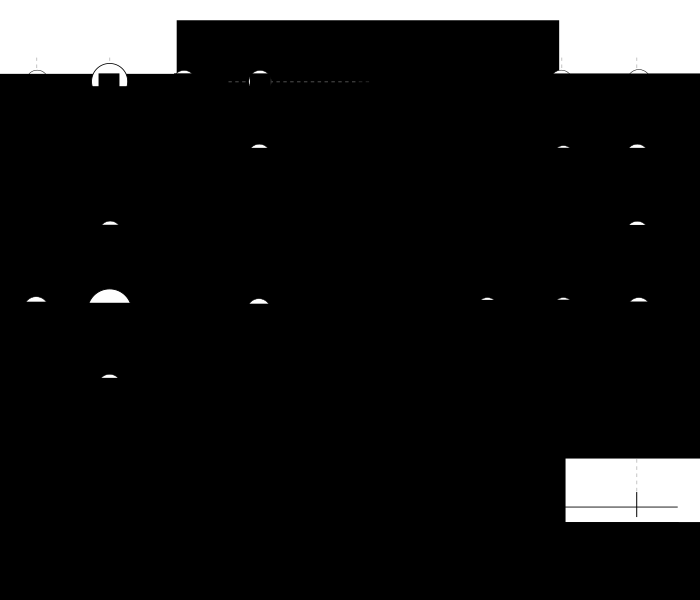
\includegraphics[width=0.75\textwidth]{figs/bubble-charts/Contribution-SLA-DIdescription.pdf}
  
\caption{Facets Contribution, SLA and Data Integration Description}\label{fig:facet1}
\end{figure} 

%  . .  .  . .  .  . .  .  . .  .  . .  .  . .  .  . .  .  . .  .  . .  .  . .  .  . .  .  . .  .  . .  .  . .  .  . .  .  . .  .  . .  .  . .  .  . .  .  . .  .  . .  .  . .  .
\textbf{\textit{RQ2: How have published papers on data integration evolved towards cloud topics?}}
%  . .  .  . .  .  . .  .  . .  .  . .  .  . .  .  . .  .  . .  .  . .  .  . .  .  . .  .  . .  .  . .  .  . .  .  . .  .  . .  .  . .  .  . .  .  . .  .  . .  .  . .  .  . .  .
\begin{figure}[h]
\centering
\includegraphics[width=0.86\textwidth]{figs/bubble-charts/DI-Environment-Contribution-Research.pdf}
\caption{Facets Data Integration Environment, Contribution and Research}\label{fig:facet2}
\end{figure}

Combining the facets data integration environment, contribution
and research it is possible to observe  the evolution of publications on data integration towards the cloud (Figure~\ref{fig:facet2}).  {\em Data warehouse} environments are the most common architecture. This can be explained by the increase of scientific  and industrial applications needing to build integrated  data sets for performing analysis and decision making tasks. The proposals are delivered as {\em models}  (14  papers - 12.27\%)  and {\em tools} (18
papers - 15.78\%)  used for facilitating data integration, mostly done in the {\em cloud}.  The most popular deployment environment of recent papers is the {\em cloud}. Given the importance and crucial need of data integration  most papers present concrete solutions as algorithms, methods and systems (31 papers - 27.19\%).
  
%  . .  .  . .  .  . .  .  . .  .  . .  .  . .  .  . .  .  . .  .  . .  .  . .  .  . .  .  . .  .  . .  .  . .  .  . .  .  . .  .  . .  .  . .  .  . .  .  . .  .  . .  .  . .  .
\textbf{\textit{RQ3:  In which way and in which context has data integration been linked to QoS measures in the literature?}}
%  . .  .  . .  .  . .  .  . .  .  . .  .  . .  .  . .  .  . .  .  . .  .  . .  .  . .  .  . .  .  . .  .  . .  .  . .  .  . .  .  . .  .  . .  .  . .  .  . .  .  . .  .  . .  .
\begin{figure}[!h]
\centering
\includegraphics[width=0.85\textwidth]{figs/bubble-charts/Data-Quality-DI.pdf}
\caption{Facets Data Quality, Data Integration Environment and Data Integration Description}\label{fig:facet4}
\end{figure}

We answered RQ3 by combining the facet {\em data quality} with the facets {\em data integration environment} and {\em data integration description}
(Figure~\ref{fig:facet4}).  Data integration and QoS measures are associated within environments like cloud  (9.68\%) and multi-cloud (4.39\%).

According to our quantitative analysis we observe that QoS has started to be
considered for integrating data. 
 The cloud is becoming a popular environment to
perform data integration in which security issues are most frequently addressed.
We identify a promising research area concerning the need of studying SLA which
is currently addressed  for the cloud as a whole \cite{PedrinaciCL14} but that
needs to be specialized for data integration aspects. Therefore, it is important
to identify the measures that characterize the quality of data and  the
quality measures associated to different phases of data integration. These phases include selecting
data services, retrieving data, integrating and correlating them and building a
query result that can be eventually stored and that must be delivered. The data integration phases are implemented by greedy algorithms and generate intermediate data that
can be stored for further use. Therefore they consume storage, computing,
processing and communication resources that have an associated economic cost. These resources 
 must ensure some QoS guarantees to data consumers. This problem seems to be
open in the domain, and we believe that it must be part of  a new vision of data
integration. We believe that it is possible to add and enhance the quality of
data integration by including SLAs.                   
 % Mapping Process %

\section{Quantitative Analysis}

\subsection{Combining the facets Contribution, SLA Usage and Data Integration Description}

\begin{figure}[h!]
\centering
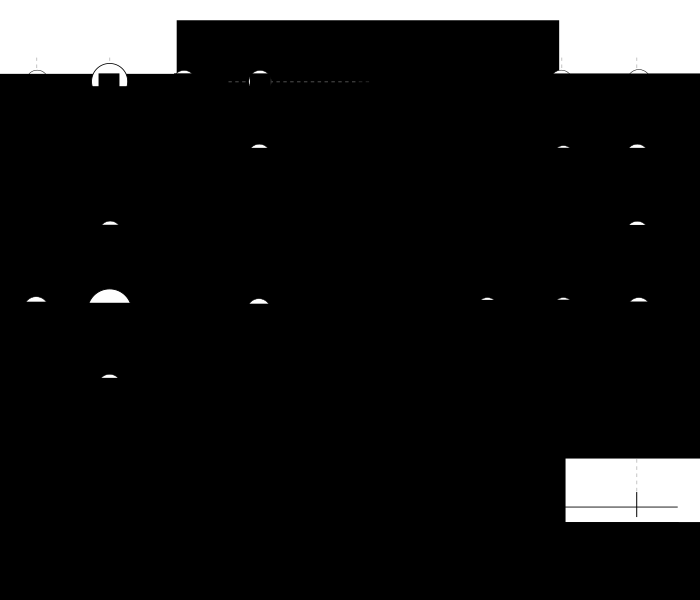
\includegraphics[scale=0.5]{figs/bubble-charts/Contribution-SLA-DIdescription.pdf} 
\caption{...}
\end{figure}

\subsection{Combining the facets Data Integration Environment, Contribution and Research}

\begin{figure}[h!]
\centering
\includegraphics[scale=0.5]{figs/bubble-charts/DI-Environment-Contribution-Research.pdf}
\caption{...}
\end{figure}

\subsection{Combining the facets SLA Usage and Contribution}

\begin{figure}[h!]
\centering
\includegraphics[scale=0.7]{figs/bubble-charts/SLA-Contribution.pdf}
\caption{...}
\end{figure}


\subsection{Combining the facets Data Quality, Data Integration Environment and Data Integration Description}

\begin{figure}[h!]
\centering
\includegraphics[scale=0.53]{figs/bubble-charts/Data-Quality-DI.pdf}
\caption{...}
\end{figure}
 % Quantitative Analysis %

%-[BEGIN]-----------------------------------------------------------------------
\section{SLA guided Data Integration on Multi-Cloud environments}\label{sec:approach}
%-[END]-----------------------------------------------------------------------
Our SLA guided data  integration approach proposes three steps starting from  query processing   to the delivery of  result sets.
Given a query and a set of QoS preferences (cost, data provenance, service reputation, execution deadline and so on), the system processes it in three steps:  (i)  {\em SLA derivation}, performed to filter possible data and services providers using a set of matching algorithms based on  graph structures and RDF specifications;
(ii)  {\em query rewriting} for computing possible service compositions giving partial or exhaustive  results according to defined SLAs; (iii)  {\em results  integration} into an answer. 
These steps generate intermediate results that are stored as knowledge  to reduce the overhead of further query evaluation processes. Moreover, an integrated SLA is generated to archive  negotiated rules obtained during  the integration. For an incoming query, the whole process is monitored to determine whether the integration SLA is being honoured.

Figure~\ref{fig_sim} shows the SLA Guided - Data Integration As A Service (SLAG-DIAAS) architecture  supported by data services which are data providers deployed in a cloud and that provide agreed SLAs. 
The SLAG-DIAAS keeps a \textit{directory} together with meta-data about the way queries are evaluated for producing results.
Query processing and monitoring modules use this information for rewriting queries according to given quality of service (QoS) preferences expressed by a data consumer.
\begin{figure}[!t]
\centering
\includegraphics[width=3in]{figs/arch}
\caption{SLAG-DIAAS architecture}
\label{fig_sim}
\end{figure}



%\section{Infrastructure implemented for the scenario}

%-[BEGIN]-----------------------------------------------------------------------
\section{Conclusion and final remarks}\label{sec:conc}

According to our classification scheme that resulted from our systematic mapping, we propose a new vision of data integration. 

\subsection{Data integration context}
We consider that data integration is done under new conditions with respect to type of data sources, the environment where it is performed and the preferences ans of data consumers and the SLA. We assume that data integration is done in the  context shown in Figure \ref{fig:vision}. 
\begin{figure}[h!]
\centering
\includegraphics[scale=0.50]{figs/DataIntegrationContext.pdf} 
\caption{New data integration context}\label{fig:vision}
\end{figure}

There are data providers that are services possibly deployed in clouds and available  through their API or in a REST architecture. We assume that  each service exports an agreed SLA that specifies the economic cost per call, the maximum number of calls that can be done per day, the availability of the service, the average response time when a method is called, the reliability, the privacy of the produced data (whether they can be stored or not), the precision of their responses, freshness and provenance of the produced data.  

%\begin{trivlist}\sf\footnotesize
%\item[~$\bullet$ ] {\sf agreedSLA:$\langle$cost/call, maxCalls/day, availability, responseTime, reliability, privacy, precision, freshness, provenance$\rangle$}. 
 %\end{trivlist}

Data integration is done on a (multi)-cloud environment. Cloud providers define also their SLA contracts expressing  subscription contracts that specify, the cost per request ({\sf cost/request}), the volume of data that can be exchanged per month ({\sf I/0 volume/month}), the cost of transferring data or applications within the same data centre or between data centres ({\sf datatransferCost/region}), and storage space ({\sf storageSpace}). For example some cloud providers enable the customer to choose the zone to install PaaS services and deploy applications (e.g. zone 1 is Europe). If the customer wishes to deploy services in zone 1 but store data in zone 2 the transfer cost will change.

%\begin{trivlist}\sf\footnotesize
 %\item[~$\bullet$ ]  {\sf cloudSLA:$\langle$cost/request, I/0 volume/month, datatransferCost/region, storageSpace$\rangle$}. 
 %\end{trivlist}


Some of these measures ({\sf cost/call, maxCall/day}) are static and explicitly specified by the service provider. 
In contrast, the other measures should be computed by monitoring the conversations between the service and the applications that contact it.  

In our vision a query expressed in an SQL-like language is associated to a set of QoS preferences (cost, data provenance, service reputation, execution deadline and so on) expressing the requirements of the user. For example, the economic cost she is ready to pay for executing the query, the provenance of the data (e.g., given by the expertise the data producers or authors), the reputation of data services and the expected time response. The answer of such a query is the result of integrating data from different services.

\subsection{SLA guided data integration}
Thus, given a query, its associated QoS preferences, cloud providers  and  services that can potentially be data providers (see Figure \ref{fig:vision}),  SLA guided data  integration can consist in three steps.  
\begin{itemize}
\item Generating a derived SLA:  
The key and original aspect of   our proposed data integration and provision process is  defined as a vertical mapping of user QoS preferences and agreed SLAs. This  leads to a {\em derived SLA} that guides the evaluation of a query. 

A query has associated preferences  expressed as macroscopic constraints (i.e. user preferences statement): execution time, pay / no pay, data reliability, provenance, freshness, privacy, partial/full results, delivery mode. These constraints are coupled with the profile of the user which is in general stated in her cloud subscription (amount of assigned storage space, number of requests, I/O transferred Mega bytes, etc.). 

Given agreed SLA's and a user preferences statement the challenge is to compute a  {\em derived SLA} that  maps SLA measures and preferences attributes.  The derived SLA is defined as a set of measures that correspond to the user preferences computed as a function of different static, computed and hybrid measures. The {\em derived SLA}  will guide the way the query will be evaluated, and the way results will be computed and delivered.
Therefore, we propose to classify SLA measures to represent the relationship between fine grained measures used by agreed SLAs and coarse grained measures used in user preferences statements. It is also necessary to specify how to compute coarse grained measures with fine grained ones. For example, data precision will be computed as a function of availability, freshness and provenance exported by data services. 

  
\item Filtering data services: the derived SLA  is used for filtering possible data services that can be used for answering the query. This is done using a set of matching algorithms based on  graph structures and RDF specifications. This step may lead either to the rejection of integration in case of total incompatibility, or to a negotiation between SLA which will lead us to the proposal for a negotiated SLA integration and thus the need for an adaptive setting.


\item   Query rewriting: Given a set of data services that can potentially provide data for integrating the query result, we compute possible data service compositions that give partial or exhaustive  results according to the derived SLA and the agreed SLA of each data service. The objective is   generate a number $k$ of service compositions, combining as much as possible the services available such that the constraints of the derived SLA are verified. 


\item  Integrating a query result: the service compositions are executed in one or several clouds where the user has a subscription. The execution cost of  service compositions must fulfill the derived SLA (that expresses user requirements). In this phase we generate an execution plan  considering the derived SLA and the subscription of the user to one or several clouds. We consider for example the economic cost determined by the data to be transferred, the number of external calls to services, data storage and results delivery costs and we decide how to use clouds resources for executing the composition. A first approach for performing this phase has been addressed  in  \cite{Lopez14}.
\end{itemize}
%These steps generate intermediate results that are stored as knowledge  to reduce the overhead of further query evaluation processes. Moreover, an integrated SLA is generated to archive  negotiated rules obtained during  the integration. For an incoming query, the whole process is monitored to determine whether the integration SLA is being honored.

%In the next sections we describe the aspects to consider for the fist two phases. 

%Figure~\ref{fig_sim} shows the SLA Guided - Data Integration As A Service (SLAG-DIAAS) architecture  supported by data services which are data providers deployed in a cloud and that provide agreed SLAs. 
%The SLAG-DIAAS keeps a \textit{directory} together with meta-data about the way queries are evaluated for producing results.
%Query processing and monitoring modules use this information for rewriting queries according to given quality of service (QoS) preferences expressed by a data consumer.
%\begin{figure}[!t]
%\centering
%\includegraphics[width=4.5in]{figs/arch}
%\caption{SLAG-DIAAS architecture}
%\label{fig_sim}
%\end{figure}

%In order to illustrate our approach, consider a smart city that aims at being energy self-sustainable and produce and consume, as much as possible, energy within its geographic area. 
%Producers are characterized according to their location, the amount of energy in Kilowatts-hour that they can sell, the cost of that energy, and the time window in which they can produce it. 
%Consumers are described by their location, their energy requirements during a certain interval of time, the maximum total cost they are ready to pay, and quality of service requirements such as availability and how critical it is to consume this amount of energy. 
%An energy exchange market is established in order to continuously trade  energy provision/consumption ensuring that all consumers will have the energy they require at every moment.


 


%In our example assume that there are several energy provision services ({\sf e$_1$, ... e$_n$}) that can be independent or hubs integrating several energy providers. 
%Each of them is specified by a clause:
%\begin{trivlist}\sf\footnotesize
%\item[~$\bullet$ ]   e$_i$ $\equiv$ provider(KW-h, Ecost, rate, location), \textit{SLA}$_i$
%\end{trivlist}

 

%According to our approach  data services have associated ``agreed'' SLAs.
% In the example, we assume that several producers will be able to supply energy for a given period of time given specific  preferences expressed by a consumer. 
%Assume that there are four household energy providers that can be queried individually and two hubs that collect information from the community smart-meters.
%Hubs will store information about (surplus) energy, available from particular users.
%We represent these services by {\sf e$_1$, \dots, e$_4$} and {\sf h$_1$ and h$_2$}.
%We also suppose the existence of two free location services exporting the following interface: {\sf loc(IP) $\leftarrow$ $\langle$ X, Y$\rangle$}, meaning that given an IP address it returns a geographic position expressed as a pair of coordinates. 
%All these services can potentially be combined for answering queries.
%
%An energy request is expressed as a query that specifies an energy requirement with QoS preferences independently of the possible producers. 
%Queries may be expressed as Datalog-like programs or an SQL-like expressions, including spatio-temporal attributes and preferences.
%For instance, \textit{List of energy providers that can provision 1000 Kwatts/h, in the next 10 seconds, that are close to my city with a cost of 0,50 euros/Kwatt and that are labeled as green?}. 
%The user preferences statement would include their cloud provider contract and quality preferences:
%
%\begin{trivlist}\sf\footnotesize
%\item[~$\bullet$ ]  {\sf cloudSLA:$\langle$0,05 cents per call, 8 Gigabytes I/0 volume/month, free, 1 Giga$\rangle$}. 
%\item[~$\bullet$ ] {\sf preferencesStatement:$\langle$query total cost,  total responseTime, reliability, freshness, precision, provenance, storage$\rangle$}. 
%\end{trivlist}
%
%
%We consider a simplified SLA cloud contract inspired in the lowest contract provided by Azure: {\sf cost of \$0,05 cents per call,  8~GB of I/O volume/month, free data transfer cost within the same region,  01~GB of storage}. 
%The user is ready to pay maximum {\sf \$5 as total query cost}; she requests that only {\sf green} energy providers are listed (provenance); at least {\sf 85$\%$} of precision of provided data, even if they are not fresh; she requires an availability rate of at least {\sf 90$\%$} and with a response time of {\sf 0,01 seconds}.
 %
%As usual, SLAs are  represented as conditions over variables that will be used in the query.
%In this context, the compliance to the SLAs will drive the query rewriting process.

%-----------------------------------------------------------------
%\subsection{Generating a derived SLA}
%\label{sec:slaModel}
%-----------------------------------------------------------------
%The key and original aspect of   our proposed data integration and provision process is  defined as a vertical mapping of user QoS preferences and agreed SLAs. This  leads to a {\em derived SLA} that guides the evaluation of a query. 

%A query has associated preferences  expressed as macroscopic constraints (i.e. user preferences statement): execution time, pay / no pay, data reliability, provenance, freshness, privacy, partial/full results, delivery mode. These constraints are coupled with the profile of the user which is in general stated in her cloud subscription (amount of assigned storage space, number of requests, I/O transferred Mega bytes, etc.). 



%One may think to a first filter to remove the individual services which do not meet some or all of the constraints expressed by the user. 

%We assume that services export SLAs (i.e., agreed SLAs) that define measures   that can be either (i) expressed as constants,  computed (dynamically) by monitoring the execution and conversations associated to services, and (ii) hybrid that can be statically stated  but they change at execution time.  A service  agreed SLA is expressed through an  XML document using the specification WSLA (Web service level agreement \footnote{\footnotesize http://www.research.ibm.com/people/a/akeller/\-Data/WSLASpecV1-20030128.pdf}). The service SLA measures  that we consider are: response time, availability, price/call, reliability, data production rate. Other measures are associated to the conditions in which the service is called or to the precision and recall of their produced data given a request. 

%An example of computed measure is the cost of retrieving the list of energy providers within a region with their KWatt cost. The cost is determined by the  cost of the calls. This request  includes the price of calling a service (e.g.,  between 0,25 - 0,50 euros depending on the data service), plus the price of data transmission according to the amount of trasnmited MegaOctets through the network and the type of subscription of the user for using the network. 
%Since we assume that services can be deployed on different cloud providers, measures and SLA threasholds can vary.

%Given agreed SLA's and a user preferences statement the challenge is to compute a  {\em derived SLA} that  maps SLA measures and preferences attributes.  The derived SLA is defined as a set of measures that correspond to the user preferences computed as a function of different static, computed and hybrid measures. The {\em derived SLA}  will guide the way the query will be evaluated, and the way results will be computed and delivered.

%In the example, some of the user preferences statement measures are used for defining a derived SLA that, as said in previous section, will guide the evaluation of the query. These measures are defined as a function of the measures used by the agreed SLAs and by the cloud SLA contract.
%\begin{trivlist}\sf\footnotesize
%\item[~$\bullet$ ] query total cost: $\sum_{i = 1\dots n}$ cost(s$_i$) + data transfer $\leq$ \$5
 %\item[~$\bullet$ ] total response time: of services + data transfer
 %\item[~$\bullet$ ] availability: {\em (of services involved)} $\leq$ {\sf 90$\%$}, 
 %\item[~$\bullet$ ] freshness: non 
 %\item[~$\bullet$ ] precision: {\em avg (precision of services involved)} $\leq$ {\sf 85$\%$}
 %\item[~$\bullet$ ] provenance:  all services involved must be $green$
 %\item[~$\bullet$ ] storage: {\em partial results size} $\leq 1$ GB
 %\end{trivlist} 
 
%Therefore, we propose a classification of SLA measures that represents the relationship between fine grained measures used by agreed SLAs and coarse grained measures used in user preferences statements. It specifies also how to compute coarse grained measures with fine grained ones. For example, data precision will be computed as a function of availability, freshness and provenance exported by data services. 
%The derived SLA  can be seen as a set of unequations that have to be solved during the execution of a service composition. Since some of them can only be determined at execution time, the decision on which services will participate in the evaluation of the query is approximated. We will discuss this issue in the next sections.


%This step may lead either to the rejection of integration in case of total incompatibility, or to a negotiation between SLA which will lead us to the proposal for a negotiated SLA integration and thus the need for an adaptive setting.
%
%
% \begin{enumerate}
%\item Computation of a global SLA given the existing possible SLA agreed by data providers that can be called for answering the query. Data providers are filtered in this way, since only those agreed SLA that can be combined into a global SLA that can fulfill the user preferences are considered for retrieving data.
%
 % 
%  \item Filter the data providers that can potentially participate in the evaluation of the query taking into consideration the preferences associated to the query.
  %
 % \item 
 %Negotiation of this type of SLA depends strongly on the request sent and the services deployed at the arrival time of the application on the cloud. This negotiation can be expensive and may not scale well.
 % \end{enumerate}

  
%-----------------------------------------------------------------
%\subsection{Query Rewriting}
%\label{sec:queryRew}
%-----------------------------------------------------------------
%Given a query and its preferences statement, the system  finds  service compositions that produce results   meeting the required constraints. This is done with a query rewriting algorithm adapted to the case where data providers are services. 
%Query rewriting is a well-known problem in the database domain.
%The problem consists in transforming an abstract query into a set (or list) of lower-level queries that can be solved by  available databases.
%Query rewriting is guided by the schema of  abstract and concrete databases.
%The answers to the lower level queries are combined in order to obtain the result to be returned to the user.

%The query rewriting problem can be generalized to the case of services.
%In this case, the query to be rewritten is seen as an abstract service composition, to be expressed in terms of concrete services.
%Query rewriting techniques have been adapted to the context of service composition~\cite{BBM10,ZLC11,CostaAMR13}. 
%In~\cite{CostaAMR13} the authors present an algorithm to automatically refine high-level specifications of service compositions into lower-level ones. 
%The method is based on the MiniCon algorithm~\cite{PH01} for query rewriting.

%The case of more general services (\textit{i.e}, services that maintain and update information) is a generalization of the information-provision case.
%Unlike the simpler case, where only the service interfaces need to be considered, the general case requires considering the functional and non-functional aspects of the query and available services.
%In this context, the \textit{Local as View} (\textit{LAV}) methods of query rewriting~\cite{Levy2000} are suitable.
%In the LAV approach, the rewriting process is guided by the specification of both the query to be rewritten and the available databases.
%The specification of the composition to be produced as well as the specification of each available service are used in the case of general services.
%These specifications may detail both the functional and non-functional behaviour of each service, including SLA.


%We propose an approach that consists in generating several translations of an abstract service specification into compositions
%over concrete  services. 
%The solutions proposed are ranked and may be coded into concrete workflows as shown in the following section.  The next example shows the main features of the approach proposed in~\cite{CostaAMR13} and that is extended in the case of SLA guided services based data integration. 

%\begin{example}[Service Refinement by Rewriting]\label{Ex:rew1}
%Let us consider the case of the smart city scenario, where particulars can participate on an energy trading pool.
%We suppose that this hypothetical city has a large number of households that sell their energy surplus to other consumers. 
%The city has four information hubs, located in four different neighbourhoods, connected to very small energy producers.
%Other producers are be contacted directly, though the services of three different cloud providers.
%Each cloud provider exports its own interfaces.
 %SLAs are defined for each individual energy provider server, each hub, and each cloud provider. 

%When an on-line consumer searches  servers to buy energy, a composed web service is generated, in order to fetch each individual or hub service and to start  energy reservation procedures.
%Depending on the location of the consumer and producers, different conditions and constraints may apply.
%Also  cloud providers  publish the conditions for using their services.
%These conditions are expressed as user preferences and SLAs.
%Additionally, other non-functional requirements (such as authentication or security requirements) may apply.

%In this context, the user  expresses an energy order, her location and payment information. A composite web service is  generated to fulfil the order.
%The generated service composition should consider the nearest providers, in accordance to the agreed SLA.

%In order to produce a personalized service composition for each user, the algorithm in~\cite{CostaAMR13} takes into account the specification of the composition (which may be produced by the user's browser, including context information).
%The specification of each available service is also considered (this specification should be given by the service provider).
%~\hfill\openbox
%\end{example}


%Given a a set of services that can possibly be composed and the derived SLA, a service composition must be produced.
%Some of the unequations of the derived SLA should be included in the service compositions that answer the query.
%In the case of our query example the following composition can be used for answering it:
%\begin{eqnarray*}
%Q_1 &\equiv&
 %  \langle X_1,Y_1\rangle = loc_1(IP), \\
%&& \langle X_2,Y_2 \rangle = loc_1(Eprovider), \\
%&& D = distance(\langle X_1,Y_1\rangle, \langle X_2,Y_2\rangle), \\
%&& \langle C_1, E_1 \rangle = e_1(\dots), \dots \langle C_4, E_4 \rangle = e_4(\dots), \\
%&& D \leq 1.5 \mathsf{Km},\ \ sum(C_1:C_4) \leq 5, \\
%&& sum(E_1:E_4) \geq 1000\ \mathsf{kw-h}, \\
%&& \mathsf{totalResponseTime}  \leq 10\ \mathsf{seg}
%\end{eqnarray*}

 
  
  %Our approach  generates a number $k$ of service compositions, combining as much as possible the services available such that the constraints of the derived SLA are verified. 
 %Yet, the algorithm should be modified to take into account the different SLAs. 
 %The next example illustrates one of the limits of the automatic composition algorithm.

%\begin{example}[Incremental queries]\label{Ex:rew2}
%Let us return to the energy trade system of Example~\ref{Ex:rew1}.
 %Suppose that the user requires to retrieve a list of star providers  daily and weekly that can deliver ``\textit{One MegaWatt-hour}''.
%In this case, each individual and hub database will be queried and the list will be produced by adding data obtained from them, until the one MegaWatt-hour capacity is reached.
%Let us suppose that, in order to minimize the the communications between servers, the lists need to be produced incrementally.
%In this case, the composition produced by the service refinement may need to include an iteration (to aggregate partial results). 
%The data produced by the warehouse servers will be processed in batch and the process will end once the list reaches the desired capacity.

%To our knowledge, the incremental production of a solution is beyond  the scope of the current methods for rewriting service compositions and represents a challenge to the area.
%~\hfill\openbox
%\end{example}


%-----------------------------------------------------------------
%\subsection{Dealing with the resources consumed by the evaluation process}
%\label{sec:queryProcessOpt}
%-----------------------------------------------------------------
 
 %Our data provision and integration approach relies on data services deployed on one or different providers and it is delivered as a DaaS. This DaaS  uses resources from a cloud and this use  is  guided by an economic model (stated in a cloud subscription) that puts a threshold on the amount of resources to be invested in a query evaluation process. It is thus important to optimize the use of these resources.
 
 %We believe that the optimization of this process can occur at two levels: first at the level of agreed SLA exported by services.  Indeed, queries requesting the same services compositions will have clauses in their SLAs that are more conditions of use of the infrastructure (i.e., not storing the data produced by a service). Instead of recomputing the derived SLA every time, we propose to store it and to reuse it for other queries. 
 
%Second, pre-calculated queries and partial results can be also stored in cache or in a persistent support. Rewriting results can be also stored and reduce execution and resources consumption time when evaluating similar queries. Storing or not such SLAs will depend on the cloud subscription of the user the issued the query (data access, intermediate storage capacity , cost of storage , etc ... ).
%Given this proposal, we identify several issues:
%- Level modeling would require a model that allows the representation of SLA integration.
%- There should also be a template for representing the requirements expressed by the user
%- A mining component to identify, from the requirements expressed in the template by the user, and before the analysis of the application, the candidate integration SLA to use or adapt according to the request. This implies mapping between property and expressed clauses being.

%As discussed in previous sections, the derived SLA associated to service compositions can have free measures that can only be evaluated at run-time. In order to do so, we assume that there is a monitoring system observing and aggregating events for computing resources consumption, execution and time cost, volumes of data transferred when services deliver results. These computations are used dynamically for instantiating free variables in the derived SLA and thus determine wether te contract is respected by the execution of a query. Since this is monitored dynamically, the evaluation of the query can be adapted if the SLA is not being respected anymore.




 % Conclusion ... %
 %-[END]-----------------------------------------------------------------------
This paper introduces the challenge of integrating data from distributed data services deployed on different cloud providers guided by service level agreements (SLA) and user preferences statements. The data integration problem is stated as a continuos data provision problem that has an associated economic cost and that uses automatic learning techniques for ensuring different qualities of delivered data (fresh, precise, partial).
Current big data settings impose to consider SLA and different data delivery models. We believe that given the volume and the complexity of query evaluation that includes steps that imply greedy computations, it is important to combine and revisit well-known solutions adapted to these contexts. We are currently developing the strategies and algorithms sketched here applied to energy consumption applications as the one described in the paper and also to elections and political campaign data integration in order to guide decision making on campaign strategies.
%% References with bibTeX database:

\bibliographystyle{plain}
\bibliography{bibliography}


\end{document}